% **************************************************************
% Hi! Edit this file for your presentation!
% **************************************************************

% ==================///==================///==================///
% ==================/// LATEX'S STUFF
% ==================///==================///==================///

\documentclass{beamer}
\usepackage{amsfonts,amsmath,oldgerm}
\usepackage{pgf-pie}
\usetikzlibrary{positioning}
\usepackage{pgfplots}
\usetheme{_statale}
\usepackage{subcaption}
\usefonttheme[onlymath]{serif}
\usepackage{algpseudocode}
\usetikzlibrary{decorations.pathreplacing,calc,tikzmark}


%\usepackage{tikz}
%\usepackage{pgfplots}
%\usepackage{pgf-pie}

%\pgfplotsset{compat=1.17}

\newcommand{\testcolor}[1]{\colorbox{#1}{\textcolor{#1}{test}}~\texttt{#1}}
\newcommand{\hrefcol}[2]{\textcolor{cyan}{\href{#1}{#2}}}
%\titlebackground*{assets/background}

% ==================///==================///==================///
% ==================/// SPLASH PAGE
% ==================///==================///==================///

\title{Modeling and Controlling Autonomous Transportation Systems in Smart Cities}
\foottitle{Modeling and Controlling ATSs in Smart Cities}
\subtitle{Master Thesis}
\course{ }
\author{
\href{mailto:luca.brodo001@stud.fh-dortmund.de}{Brodo Luca}
%\href{mailto:luzius.moll@polytechnique.edu}{Moll Luzius\hspace{10pt}}
%\href{mailto:riccardo.inghilleri@polytechnique.edu}{Inghilleri Riccardo}
}
%\IDnumber{7215156}

% ==================///==================///==================///
% ==================/// START PRESENTATION
% ==================///==================///==================///

\begin{document}
\maketitle
\pgfplotsset{compat = 1.3}

\footlinecolor{maincolor}

% ==================///==================///==================///
% ==================/// BODY'S PRESENTATION
% ==================///==================///==================///

\section{Why Autonomous Transportation Systems?}
% ==================///==================///==================///
\begin{frame}{Traffic Management is Necessary }
	As vehicle ownership increases, so do traffic inefficiencies. 
	\vspace{0.5cm}
	\begin{itemize}
		\item Increased congestions $\rightarrow$ toll on the economy (1\% GDP of US (\cite{schrank2012}) )
		\item Increase consumption and pollution (60\% of $\text{CO}_2$ emissions in the EU (\cite{eea2023}))
		\item Elevated risk for travellers' safety
	\end{itemize}
\end{frame}


% ==================///==================///==================///
\begin{frame}{Personalized and Shared Mobility as a solution }
	Some notable directions, such as 
	
	\begin{itemize}
		\item  Car Sharing (e.g. Car2Go)
		\item Mobility-as-a-Service (Maas) (\cite{tomaino2020maas})
		\item Autonomous Mobility on Demand (AMoD) (\cite{amod_review}, \cite{zhang2016})
		\begin{itemize}
			\item[ ] Key idea $\Rightarrow$ Holistic control over the vehicle's fleet
		\end{itemize}
	\end{itemize}
	$\rightarrow$ Next step : Autonomous Transportation Systems (ATSs) 
	
\end{frame}

%\citepaperofs{8917521}{Zgraggen}, \citepaperofs{8938759}{Carron}, \citepaperof{zhang2016}{Zhang}

% ==================///==================///==================///
\begin{frame}{ATSs: The next step }
	Extend the concept of personalized and shared mobility to goods delivery.\\
	Three main pillars 
	\vspace{0.3cm}
	\begin{itemize}
		\item Minimized environmental impact and operational costs
		\item Ensured optimal quality of service (QoS), traffic control and road usage
		\item Tailorable solution
	\end{itemize}
	$\rightarrow$ What needs to be solved?
\end{frame}

\section{Addressing Key Challenges of ATS}
%=======================================================================
% Dispatching
%=======================================================================
\begin{frame}[label=challenge]{Tackling 4 Main Challenges}
	\begin{columns}
		\begin{column}{0.4\textwidth}
			\begin{itemize}
				\item \textbf{AV Dispatching}
				\item AV Routing
				\item AV Rebalancing
				\item Ride-Sharing and Delivery Pooling
			\end{itemize}
		\end{column}
		%%
		\begin{column}{0.6\textwidth}
			\begin{figure}
				\resizebox{0.7\textwidth}{!}{
				\begin{tikzpicture}[>=stealth]
					
					% Define clients nodes
					\node[inner sep=0pt] (client1) at (-3,2.5) {\includegraphics[width=1.1cm]{img/client.png}};
					\node[inner sep=0pt] (client2) at (0,2.5) {\includegraphics[width=1.1cm]{img/client.png}};
					\node[inner sep=0pt] (client3) at (3,2.5) {\includegraphics[width=1.1cm]{img/client.png}};
					\node[inner sep=0pt] (client4) at (-4,0) {\includegraphics[width=1.1cm]{img/client.png}};
					\node[inner sep=0pt] (client5) at (-1,0) {\includegraphics[width=1.1cm]{img/goods.png}};
					\node[inner sep=0pt] (client6) at (1,0) {\includegraphics[width=1.1cm]{img/goods.png}};
					\node[inner sep=0pt] (client7) at (4,0) {\includegraphics[width=1.1cm]{img/goods.png}};
					
					% Define AVs nodes
					\node[inner sep=0pt] (AV1) at (-3,-3) {\includegraphics[width=2.4cm]{img/car.png}};
					\node[inner sep=0pt] (AV2) at (0,-3) {\includegraphics[width=2.4cm]{img/car.png}};
					\node[inner sep=0pt] (AV3) at (3,-3) {\includegraphics[width=2.4cm]{img/car.png}};

					
					% Arrows from clients to AVs
					\draw[->] (client1.south) -- (AV1.north);
					\draw[->] (client2.south) -- (AV2.north);
					\draw[->] (client3.south) -- (AV3.north);
					\draw[->] (client4.south) -- (AV1.north);
					\draw[->] (client5.south) -- (AV2.north);
					\draw[->] (client6.south) -- (AV2.north);
					\draw[->] (client7.south) -- (AV3.north);
					
					% Label clients and AVs
					\node[above=0.2cm of client1] {Client 1};
					\node[above=0.2cm of client2] {Client 2};
					\node[above=0.2cm of client3] {Client 3};
					\node[above=0.2cm of client4] {Client 4};
					\node[above=0.2cm of client5] {Client 5};
					\node[above=0.2cm of client6] {Client 6};
					\node[above=0.2cm of client7] {Client 7};
					\node[below=0.2cm of AV1] {AV 1};
					\node[below=0.2cm of AV2] {AV 2};
					\node[below=0.2cm of AV3] {AV 3};

					
				\end{tikzpicture}
				
			}
			\end{figure}
		\end{column}
	\end{columns}
\end{frame}

\addtocounter{framenumber}{-1}
%=======================================================================
% Routing
%=======================================================================
\begin{frame}[label=challenge]{Tackling 4 Main Challenges}
	\begin{columns}
		\begin{column}{0.4\textwidth}
			\begin{itemize}
				\item AV Dispatching
				\item \textbf{AV Routing}
				\item AV Rebalancing
				\item Ride-Sharing and Delivery Pooling
			\end{itemize}
		\end{column}
		%%
		\begin{column}{0.6\textwidth}
			\begin{figure}
				\resizebox{0.9\textwidth}{!}{
				\begin{tikzpicture}[>=stealth]
					% Define places nodes
					\node[circle, draw, minimum size=1.5cm] (place1) at (-3,2) { 1};
					\node[circle, draw, minimum size=1.5cm] (place2) at (0,2) { 2};
					\node[circle, draw, minimum size=1.5cm] (place3) at (3,2) { 3};
					\node[circle, draw, minimum size=1.5cm] (place4) at (-4,-1) { 4};
					\node[circle, draw, minimum size=1.5cm] (place5) at (-1,-1) { 5};
					\node[circle, draw, minimum size=1.5cm] (place6) at (1,-1) { 6};
					\node[circle, draw, minimum size=1.5cm] (place7) at (4,-1) { 7};
					
					% Arrows for roads
					\draw[->] (place1) -- (place2);
					%\draw[->] (place2) -- (place3);
					\draw[->] (place1) -- (place4);
					%\draw[->] (place4) -- (place5);
					\draw[->] (place5) -- (place6);
					\draw[->] (place2) -- (place6);
					\draw[->] (place6) -- (place7);
					\draw[->] (place7) -- (place3);
					
					%\draw[->,] (place4) -- (place5) node[midway,above,sloped] {\includegraphics[width=1cm]{img/car.png} };
					\draw[->] (place4) -- node[midway, above, sloped] {\includegraphics[width=1cm]{img/car.png}} node[midway, above=0.8cm] {\includegraphics[width=0.5cm]{img/goods.png}} (place5);
					
					%\draw[->,] (place2) -- (place3) node[midway,above,sloped] {\includegraphics[width=1cm]{img/car.png} };
					\draw[->] (place2) -- node[midway, above, sloped] {\includegraphics[width=1cm]{img/car.png}} node[midway, above=0.8cm] {\includegraphics[width=0.5cm]{img/client.png}} (place3);
					
					
					%\draw[->,] (place7) -- (place3) node[midway,above,sloped] {\includegraphics[width=1cm]{img/car.png} };
					\draw[->] (place6) -- node[midway, above, sloped] {\includegraphics[width=1cm]{img/car.png}} node[midway, above=0.8cm] {\includegraphics[width=0.5cm]{img/goods.png}} (place7);
					
					% Define AVs nodes
					%\node[inner sep=0pt] (AV1) at (-2.25,0.5) {\includegraphics[width=1cm]{img/car.png}};
					%\node[inner sep=0pt] (AV2) at (0,0.5) {\includegraphics[width=1cm]{img/car.png}};
					%\node[inner sep=0pt] (AV3) at (2.25,0.5) {\includegraphics[width=1cm]{img/car.png}};
					
				\end{tikzpicture}
					
				}
			\end{figure}
		\end{column}
	\end{columns}
\end{frame}


\addtocounter{framenumber}{-1}
%=======================================================================
% Rebalancing
%=======================================================================
\begin{frame}[label=challenge]{Tackling 4 Main Challenges}
	\begin{columns}
		\begin{column}{0.4\textwidth}
			\begin{itemize}
				\item AV Dispatching
				\item AV Routing
				\item \textbf{AV Rebalancing}
				\item Ride-Sharing and Delivery Pooling
			\end{itemize}
		\end{column}
		%%
		\begin{column}{0.6\textwidth}
			\begin{figure}
				\resizebox{0.7\textwidth}{!}{
					\begin{tikzpicture}[>=stealth]
						% Define places nodes
						\node[circle, draw, minimum size=1.5cm] (place1) at (-3,2) { 1};
						\node[circle, draw, minimum size=1.5cm] (place2) at (0,2) { 2};
						\node[circle, draw, minimum size=1.5cm] (place3) at (3,2) { 3};
						\node[circle, draw, minimum size=1.5cm] (place4) at (-4,-1) { 4};
						\node[circle, draw, minimum size=1.5cm] (place5) at (-1,-1) { 5};
						\node[circle, draw, minimum size=1.5cm] (place6) at (1,-1) { 6};
						\node[circle, draw, minimum size=1.5cm] (place7) at (4,-1) { 7};
						
						% Arrows for roads
						%\draw[->] (place1) -- (place2);
						\draw[->] (place2) -- (place3);
						%\draw[->] (place1) -- (place4);
						\draw[->] (place4) -- (place5);
						\draw[->] (place5) -- (place6);
						\draw[->] (place6) -- (place7);
						\draw[->] (place7) -- (place3);
						
						\draw[->,] (place2) -- (place6) node[midway,above,sloped] {\includegraphics[width=1cm]{img/car.png} };
						
						
						\draw[->,] (place1) -- (place2) node[midway,above,sloped] {\includegraphics[width=1cm]{img/car.png} };
						
						
						
						\draw[->,] (place1) -- (place4) node[midway,above,sloped, xscale=-1] {\includegraphics[width=1cm]{img/car.png} };
						
						
						% Define AVs nodes
						%\node[inner sep=0pt] (AV1) at (-2.25,0.5) {\includegraphics[width=1cm]{img/car.png}};
						%\node[inner sep=0pt] (AV2) at (0,0.5) {\includegraphics[width=1cm]{img/car.png}};
						%\node[inner sep=0pt] (AV3) at (2.25,0.5) {\includegraphics[width=1cm]{img/car.png}};
						
					\end{tikzpicture}
					
				}
			\end{figure}
		\end{column}
	\end{columns}
\end{frame}


\addtocounter{framenumber}{-1}
%=======================================================================
% Ride-Sharing
%=======================================================================
\begin{frame}[label=challenge]{Tackling 4 Main Challenges}
	\begin{columns}
		\begin{column}{0.4\textwidth}
			\begin{itemize}
				\item AV Dispatching
				\item AV Routing
				\item AV Rebalancing
				\item \textbf{Ride-Sharing and Delivery Pooling}
			\end{itemize}
		\end{column}
		%%
		\begin{column}{0.6\textwidth}
			\begin{figure}
				\resizebox{0.9\textwidth}{!}{
					\begin{tikzpicture}[>=stealth]
						
						% Define clients nodes
						\node[inner sep=0pt] (client2) at (0,2.5) {\includegraphics[width=1.1cm]{img/client.png}};
						\node[inner sep=0pt] (client5) at (-1,0) {\includegraphics[width=1.1cm]{img/goods.png}};
						\node[inner sep=0pt] (client6) at (1,0) {\includegraphics[width=1.1cm]{img/goods.png}};
						
						% Define AVs nodes
						\node[inner sep=0pt] (AV2) at (0,-3) {\includegraphics[width=2.4cm]{img/car.png}};
						
						% Arrows from clients to AVs
						\draw[->] (client2.south) -- (AV2.north);
						\draw[->] (client5.south) -- (AV2.north);
						\draw[->] (client6.south) -- (AV2.north);
						
						% Label clients and AVs
						\node[above=0.2cm of client2] {Client 1};
						\node[above=0.2cm of client5] {Client 2};
						\node[above=0.2cm of client6] {Client 3};
						\node[below=0.2cm of AV2] {AV};
						
						\node[circle, draw, minimum size=1.5cm] (place1) at (5,1) { 1};
						\node[circle, draw, minimum size=1.5cm] (place2) at (8,1) { 2};
						\node[circle, draw, minimum size=1.5cm] (place3) at (11,1) { 3};
						\node[circle, draw, minimum size=1.5cm] (place7) at (13,-1) { 7};
						
						
						\draw[->] (place1) -- (place2);
						\draw[->] (place2) -- (place3);
						\draw[->] (place3) -- (place7);
						
						\node[left=0.2cm of place1, scale=4] {$\Rightarrow$};
						
						
						\node[inner sep=0pt] (client2a) at (place2)[above=1cm] { \includegraphics[width=1.1cm]{img/client.png}};
						\node[inner sep=0pt] (client5a) at (place3)[above=1cm]{ \includegraphics[width=1.1cm]{img/goods.png}}; % Placed above place1
						\node[inner sep=0pt] (client6a) at (place7)[above=1cm]{ \includegraphics[width=1.1cm]{img/goods.png}}; % Placed above place3
						\node[above=0.2cm of client2a] {Client 1};
						\node[above=0.2cm of client5a] {Client 2};
						\node[above=0.2cm of client6a] {Client 3};
					\end{tikzpicture}
					
				}
			\end{figure}
		\end{column}
	\end{columns}
\end{frame}

\addtocounter{framenumber}{-1}

\section{Modeling and Managing ATSs - The CATSM Problem} 

% ==================///==================///==================///
\begin{frame}{How to tackle them?}
	By observing what we have. \\
	
	\vspace{0.5cm}
	\begin{itemize}
		\item Road Network
		\item Vehicles
		\item Requests
	\end{itemize}
	\vspace{0.5cm}
	$\rightarrow$ Creating a vehicle-centric model of the ATS to solve the challenges.
\end{frame}

% ==================///==================///==================///
\begin{frame}{Modeling the Road Network}
	Using a uni-directed graph $\mathcal{G} = \langle \mathcal{V}, \mathcal{E} \rangle$, where $\mathcal{V}$ represents the set of vertices (locations) and $\mathcal{E} \subseteq \mathcal{V} \times \mathcal{V}$ represents the edges (roads).
	\vspace{0.5cm}
	\begin{itemize}
		\item Each edge is associated with multiple metrics (e.g., distance $d: \mathcal{E} \rightarrow \mathbb{R}_{\geq 0}$).
		\begin{itemize}
			\item[ ] $\Rightarrow$ Artificial limit on number of vehicles at each time
		\end{itemize}
		\item Nodes can be of two types: charging ($\mathcal{V}_c$) and normal ($\mathcal{V}_n$) nodes.
		\item Charging nodes using ad-hoc charging profile models.
	\end{itemize}
\end{frame}


% ==================///==================///==================///

%\begin{frame}{Charging Profiles}
%	 	\vspace{0.1cm}
%	AV batteries modeled as tuple  $\mathcal{T}_a =\langle Q_a, I^b_a, R^-_a, R^+_a,\theta_a\rangle$. \\
%	Using the CC-CV (Constant current - Constant Voltage) scheme. 
%	\vspace{0.1cm}
%	\input{img/half_battery_profiles}
%\end{frame}

% ==================///==================///==================///

\begin{frame}{Modeling AVs}
	Each vehicle $a \in\mathcal{A}$ having: %as a tuple $\langle \underline{s_a},\bar{t_a}, B_a(t),\mathcal{R}_a, \mathcal{T}_a, P_a, G_a, C_a, F_a  \rangle$.
	\begin{itemize}
		\item Starting and terminating nodes $\underline{s_a}$ and $\bar{t_a}$ 
		\item  State of Charge $B_a \in \mathbb{R}_{>0}$ at time $t$
		\item  Goods and people capacity $G_a \in \mathbb{R}_{\ge0}$ and $P_a \in \mathbb{R}_{\ge0}$ 
		\item  Operational cost $C_a \in \mathbb{R}_{>0}$ 
		\item  Pollution factor $F_a \in \mathbb{R}_{>0}$
		%\item A battery $\mathcal{T}_a$
		%\item Charging and discharching rate $R^-_a, R^+_a$ 
		\item Set of assigned requests $\mathcal{R}_a$ 
	\end{itemize}
\end{frame}




\begin{frame}{Modeling Requests}
	Requests are modeled according to%as tuples $\langle \underline{s'},\bar{t'}, G', P',\lambda, a', b'\rangle$
	\begin{itemize}
		\item  Pick-up and drop-off nodes $\underline{s'} \in \mathcal{V}_n$ and $\bar{t'} \in \mathcal{V}_n$ 
		\item  Transportation demands for goods and people $G'\in \mathbb{R}_{\ge0}$ $P'\in \mathbb{R}_{\ge0}$ 
		\item  Deterministic arrival rate $\lambda \in \mathbb{R}_{>0}$ 
		\item  Time window $[a',b']$ 
	\end{itemize}
\end{frame}



% ==================///==================///==================///

\begin{frame}{The Complete ATS Management Problem}
	%Informally, the Complete ATS Management Problem (CATSM) maximizes number of served requests and minimize vehicle's travel time, while
	Combine the three models to
	\begin{itemize}
		\item Maximize number of served requests
		\item Reduce travel time (and pollution)
	\end{itemize}
	while
	\begin{itemize}
		\item Respecting deadlines
		\item Observing vehicle's characteristics (e.g., charge, cost and capacity)
		\item  Eliminating congestions $\rightarrow$ artificial limit $c$ on vehicles per road.
	\end{itemize}
		\vspace{0.5cm}
	$\rightarrow$ Naturally an optimization problem.
	
\end{frame}
% ==================///==================///==================///

\begin{frame}{Simulating the CATSM in Real-World}
	 \begin{columns}
	 		\begin{column}{0.37\textwidth}
	 			Using real-world data from NYC\\
	 			\begin{itemize}
	 				\item Geo-limited
	 				\item Large road network ($|\mathcal{V}|=$~500, $|\mathcal{E}|=$1700 )
	 				\item Deterministic $\lambda$s %requests rates
	 	 		\end{itemize}
	 		\end{column}
	 			\begin{column}{0.44\textwidth}
	 			\begin{figure}[tbh]
	 				\centering
	 				\begin{tikzpicture}[node distance=0cm]
	 					\node (left) at (0,-1) {\includegraphics[width=0.45\textwidth]{img/new_york_vanilla_info.png}};
	 					\node[right=0.1cm of left, scale=2] {$\Rightarrow$};
	 					\node (right) at (4,-1) {\includegraphics[width=0.45\textwidth]{img/new_york_simplified_roads.png}};
	 				\end{tikzpicture}
	 			\end{figure}
	 			\vspace{0.5cm}
	 		\end{column}
	 \end{columns}
\end{frame}


% ==================///==================///==================///
\begin{frame}{Evaluation}
	\hspace{0.5cm} Promising results, but interrogatives are left open. 
	\vspace{0.5cm}
	\begin{columns}
		\begin{column}{0.35\textwidth}
			
			\begin{itemize}
				\item[+] Solves all the challenges
				\item[+] Reduced computation thanks to a clever rebalancing formulation
				%\item[+] Numerically optimal solutions
				\item[+] Flexible and Modular model
			\end{itemize}
		\end{column}
		%%
		\vline
		\hspace{0.8cm}
		\begin{column}{0.4\textwidth}
			\begin{itemize}
				\item[-] Congestion model is highly simplified
				\item[-] Suffers large networks 
				%\item[-] Not suitable for real-time 
				\item[-] Does not gain insights on the future
			\end{itemize}
		\end{column}
	\end{columns}
\end{frame}
\section{Modeling and Controlling ATSs - The MPC for ATS and the RCS} 

% ==================///==================///==================///
\begin{frame}{How can the CATSM shortcomings be solved?}
	Three combined approaches
	\vspace{0.5cm}
	\begin{itemize}
		\item Novel linear discrete-time model
		\item Definition of an ad-hoc model predictive control (MPC) 
		\item Adaptive road network optimization using graph transformation systems (GTS)
	\end{itemize}
\end{frame}

% ==================///==================///==================///
\begin{frame}{Novel Model for ATSs}
	Key idea $\rightarrow$ Define AVs speed in function of the number of AVs currently on the street
	\begin{columns}
		\begin{column}{0.4\textwidth}
			\begin{equation*}
				\resizebox{1.3\textwidth}{!}{$
				\begin{aligned}	
					s_{ij}(V_{ij}) &= \begin{cases}
						l_{ij} \quad\quad &\text{if } V_{ij}\in[0,V_{ij}^{th})\\ 
						l_{ij} - b\cdot(V_{ij}^{th}- V_{ij}) \quad\quad &\text{if }V_{ij}\in[V_{ij}^{th}, V_{ij}^{max})\\ 
						0\quad\quad &\text{if }V_{ij} \ge V_{ij}^{max}\\ 
					\end{cases}\\
					\text{with } b  &=  \dfrac{l_{ij}-\epsilon }{ V_{ij}^{th} -  V_{ij}^{max}} \text{ and } \epsilon \in (0,1)
				\end{aligned}
				$}
			\end{equation*}
			$\rightarrow$ Implicitely, a better congestion model
		\end{column}
		\begin{column}{0.4\textwidth}
			\begin{figure}[t]
				\centering
				\resizebox{1.1\textwidth}{!}{
				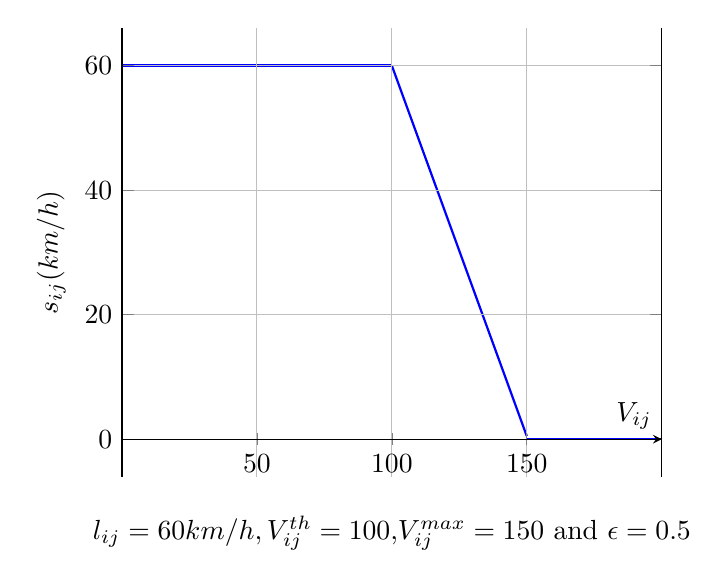
\begin{tikzpicture}
					\begin{axis}[
						xlabel={$V_{ij}$},
						ylabel={$s_{ij} (km/h)$},
						domain=0:250, % adjust the domain based on your preference
						samples=40,
						grid=both,
						axis x line=middle,
						%ymin=-1, % Set the minimum y-axis value
						%ymax=1.4, % Set the maximum y-axis value
						axis on top,
						legend pos=north east,
						title style={at={(0.5,-0.1)},anchor=north,yshift=-0.5},
						title={$l_{ij} = 60 km/h,V_{ij}^{th} = 100$,$V_{ij}^{max} = 150$ and $\epsilon = 0.5$},
						]
						% Piecewise function
						\addplot[blue, thick, domain=0:100] {60};
						\addplot[blue, thick, domain=100:150] {60 - 1.19*(x-100)};
						\addplot[blue, thick, domain=150:200] {0};
						%\addlegendentry{B}
					\end{axis}
				\end{tikzpicture}
			}
			\end{figure}
		\end{column}
	\end{columns}
\end{frame}

% ==================///==================///==================///
\begin{frame}{Novel Model for ATSs}
	As a result, new model linear time-discrete model can be defined, which tracks
	\begin{itemize}
		\item AVs' position using the speed 
		\item Stationed AVs
		\item Served and Unrequests using travelling vehicles
	\end{itemize}
	\vspace{0.3cm}
	$\rightarrow$ It's also easily controllable
\end{frame}

% ==================///==================///==================///
\begin{frame}{MPC for ATSs}
	Let $V_{ij}(t) \in \{ x \in \mathbb{N}_0 : x \leq |\mathcal{A}|\}$ being the total number of vehicles currently circulating on the street $\langle i,j\rangle$, this can be easily computed by adding the number of carries to the rebalancing AVs, i.e. \\
	\begin{equation*}
		V_{ij}(t) = \sum_{a \in \mathcal{A}} v^{a}_{ij}(t) +w^{a}_{ij}(t)
	\end{equation*}
	$\rightarrow$ Control  $v^{a}_{ij}(t)$ and $w^{a}_{ij}(t)$
\end{frame}
% ==================///==================///==================///
\begin{frame}{MPC for ATSs}
	Let $\mathcal{X}$ and $\mathcal{U}$ being the set of feasible states and inputs, respectively, solve
	\begin{equation}
		\begin{aligned}
			\underset{\substack{u(t), \dots, u(t+N)}}{\text{\textbf{min}}} \quad & J_f(x(N))+\sum_{t=0}^{N-1}I(x(t)) \\
			\text{\textbf{s.t.}} \quad & x(t+1) = Ax(t) + Bu(t)  \\
			& x(t) \in \mathcal{X}, \ u(t)\in \mathcal{U} \\
			%& k = t, \dots, t+N\\
			&x(N) \in \mathcal{X}_f\\
		\end{aligned}
	\end{equation}
	where $\mathcal{X}_f$ is the set of terminal states, $J_f(x(N))$ is the terminal cost function and $I(x(t))$ is the stage cost
\end{frame}
% ==================///==================///==================///
\begin{frame}{MPC for ATSs}
The main objectives are to:
\vspace{0.1cm}
\hspace{9.5 cm}\tikzmark{right}
\begin{itemize}
	\item Reduce number of outstanding requests \tikzmark{a}
	\item Minimize unnecessary rebalancing vehicles \tikzmark{b}
	\vspace{0.2cm}
	\item Avoid transportation after requests are served \tikzmark{c}
	\item Avoid rebalancing after requests are served \tikzmark{d}
\end{itemize}
\vspace{0.7cm}
$\rightarrow$ Stability can be proven

\begin{tikzpicture}[overlay, remember picture]
	\node[anchor=base] (1) at (pic cs:a) {\vphantom{h}}; % push the mark to the top of the line (ie including ascenders)
	\node[anchor=base] (2) at (pic cs:b) {\vphantom{g}}; % push the mark to the bottom of the line (ie including descenders)
	\node[anchor=base] (3) at (pic cs:c) {\vphantom{h}}; % push the mark to the top of the line (ie including ascenders)
	\node[anchor=base] (4) at (pic cs:d) {\vphantom{g}}; % push the mark to the bottom of the line (ie including descenders)
	\draw [decoration={brace,amplitude=0.5em},decorate,ultra thick,black]
	(1.north -| {pic cs:right}) -- (2.south -| {pic cs:right}) node[midway, right=1em] {Combined give $I(x(t))$};
	\draw [decoration={brace,amplitude=0.5em},decorate,ultra thick,black]
	(3.north -| {pic cs:right}) -- (4.south -| {pic cs:right}) node[midway, right=1em] {Combined give $J_f(x(N))$};
\end{tikzpicture}
\end{frame}
% ==================///==================///==================///
\begin{frame}{Reduced Connectivity Schema}
	As a result, a more sophisticated congestion model and insights on the impact of the decisions on the future have been acquired.What about real-time and scalability?\\
	\vspace{0.5cm}
	Solution: Reduced Connectivity Schema (RCS)\\
	In a nutshell $\rightarrow$ Create a simplified version of $G$  using a sequence of transformation rules $\mathcal{T}$.
\end{frame}
% ==================///==================///==================///
\begin{frame}{Constructing an RCS}
	Rules are highly application-dependent, therefore let's assume the NYC road network used prior. \\
	\vspace{0.2cm}
	Examples of applied rules starting from only the important nodes
	\begin{enumerate}
		\item Restoration of important nodes' immidiate connections 
		\item Restoration of simpe nodes' immidiate connections (iteratively)\label{rule2}
		\item Straight Line Node elimination
		\item Dead-End Removal
	\end{enumerate}
	\vspace{0.2cm}
	$\rightarrow$ Depending on rule \ref{rule2}, the RCS may comprise as little as 18\% of the original road network's size.
	
\end{frame}

% ==================///==================///==================///
\begin{frame}{Evaluating the MPC performance}
	\begin{columns}
		\begin{column}{0.4\textwidth}
			\begin{table}
			\begin{tabular}{ |l| c|c|c|}
				\cline{2-4}
				\multicolumn{1}{c|}{}&\multicolumn{2}{c|}{No RCS}& RCS\\
				\cline{2-4}
				\multicolumn{1}{c|}{}& 1 &  2&3\\
				\cline{1-4}
				AVs \#& 30&-&-\\
				Horizon (h) & 3 &-& -\\
				Threshold (km/h) & 60&-&-\\
				Requests & 240&-&-\\
				Road (km) & 30&R&-\\
			\end{tabular}
		\end{table}
		\end{column}
		\begin{column}{0.4\textwidth}
			\begin{table}
			\begin{tabular}{ |p{2.9cm}|c|c|c|}
				\cline{2-4}
				\multicolumn{1}{c|}{}&\multicolumn{2}{c|}{No RCS}& RCS\\
				\cline{2-4}
				\multicolumn{1}{c|}{}& 1 &  2&3\\
				\cline{1-4}
				ATT	(\%)		&33&36& 3\\
				ART	(\%)		&17&14 &3\\
				Required AVs			&19&12& 10\\
				Carrying AVs			&13&11&4\\
				Rebalancing AVs			&11&12 &9\\
			\end{tabular}
		\end{table}
		\end{column}
	\end{columns}
\end{frame}
% ==================///==================///==================///
\begin{frame}{Evaluating the MPC performance}
	\begin{figure}[t]
		\centering
		\resizebox{0.9\textwidth}{!}{
		\begin{tikzpicture}
			\begin{axis}[
			xlabel={$N$},
			ylabel={$\text{Vehicle Usage}$},
			xmin=0, xmax=20,
			ymin=-2, ymax=25,
			xtick={0,2,4,6,8,10,12,14,16,18,20,22},
			%ytick={0,1,2,3,4,5,6,7,8,9,10,11,12,13,14,15,16,17,18,19,20},
			grid=both,
			minor tick num=1,
			width=10cm,
			height=7cm,
			%ymajorgrids=true,
			%grid style=dashed,
			%mark=*,
			%mark options={blue},
			%legend style={at={(0.5,-0.15)},anchor=north,legend columns=-1},
			%legend style={at={(0.5,-0.15)},anchor=north,legend columns=-1, font=\footnotesize},
			legend style={
				at={(1.5,0.5)},
				anchor=east,
				legend columns=1
				legend image post style={scale=0.8} % Adjust the scale as needed
			},
			%legend entries={Plot 1, Plot 2, Plot 3, Plot 4, Plot 5},
			]
			\addplot[viridisbluecolor, mark=*] coordinates {
				(0,0) (1,20) (2,20) (3,20) (4,20) (5,20) (6,20) (7,20) (8,20) (9,20) (10,20) (11,20) (12,20) (13,0) (14,4) (15,3) (16,0) (17,0) (18,3) (19,1) (20,0)(21,0) (22,0)
			};
			\addlegendentry{$i=3, r = 30$}
			\addplot[viridismagentacolor, mark=+] coordinates {
				(0,0) (1,20) (2,20) (3,20) (4,20) (5,20) (6,20) (7,20) (8,20) (9,20) (10,20) (11,20) (12,20) (13,20) (14,15) (15,13) (16,4) (17,6) (18,3) (19,1) (20,0)(21,0) (22,0)
			};
			\addlegendentry{$i=3, r = 60$}
			\addplot[viridisorangecolor, mark=o] coordinates {
				(0,0) (1,20) (2,20) (3,20) (4,20) (5,20) (6,20) (7,20) (8,20) (9,20) (10,20) (11,20) (12,20) (13,18) (14,14) (15,5) (16,8) (17,6) (18,8) (19,5) (20,0)(21,0) (22,0)
			};
			\addlegendentry{$i=3, r = 90$}
			\addplot[viridiscyancolor, mark=x] coordinates {
				(0,0) (1,20) (2,20) (3,20) (4,20) (5,20) (6,20) (7,20) (8,20) (9,20) (10,20) (11,20) (12,20) (13,20) (14,20) (15,20) (16,18) (17,9) (18,7) (19,2) (20,0) (21,0) (22,0)
			};
			\addlegendentry{$i=3, r = 120$}
			\addplot[viridisgreencolor,mark=square] coordinates {
				(0,0) (1,20) (2,20) (3,20) (4,20) (5,20) (6,20) (7,20) (8,20) (9,20) (10,20) (11,20) (12,20) (13,20) (14,20) (15,20) (16,18) (17,9) (18,7) (19,2) (20,0) (21,0) (22,0)
			};
			\addlegendentry{$i=2, r = 150$}
			
			\addplot[viridisbluecolor,mark=square] coordinates {
				(0, 0) (1, 20) (2, 20) (3, 20) (4, 20) (5, 20) (6, 20) (7, 20) (8, 20) (9, 20) (10, 20) (11, 20) (12, 20) (13, 20) (14, 20) (15, 18) (16, 12) (17, 10) (18, 9) (19, 3) (20, 0)
			};
			\addlegendentry{$i=2, r = 180$}
			\addplot[viridismagentacolor,mark=square] coordinates {
				(0, 0) (1, 16) (2, 16) (3, 16) (4, 16) (5, 16) (6, 16) (7, 16) (8, 16) (9, 16) (10, 16) (11, 16) (12, 16) (13, 16) (14, 16) (15, 16) (16, 16) (17, 16) (18, 14) (19, 2) (20, 0)
			};
			\addlegendentry{$i=2, r = 210$}
			\addplot[viridispurplecolor,mark=square] coordinates {
				(0, 0) (1, 20) (2, 20) (3, 20) (4, 20) (5, 20) (6, 20) (7, 20) (8, 20) (9, 20) (10, 20) (11, 20) (12, 20) (13, 20) (14, 20) (15, 20) (16, 19) (17, 14) (18, 8) (19, 2) (20, 0)
			};
			\addlegendentry{$i=4, r = 210$}
		\end{axis}
		
		
			
			
		\end{tikzpicture}
	}
	\end{figure}
\end{frame}





% ==================///==================///==================///
% ==================/// END PRESENTATION
% ==================///==================///==================///

%\backmatter

\begin{frame}{Summary and Outlook}	
	On the one hand, promising fundations have been layed down
	\vspace{0.15cm}
	\begin{itemize} 
		\item Holistic model for an ATS leading to a complete solution of its challenges
		\item Modular, adaptable and efficient linear model for real-time application
		\item Definition of a stable MPC for optimal control
		\item Novel complexity-reduction technique proposed for the road-network representation
	\end{itemize}
	\vspace{0.15cm}
	On the other, multiple research directions have been opened:
	\vspace{0.15cm}
	\begin{itemize} 
		\item GTS must be further explored for more applications
		\item Using the MPC to control real-world vehicles 
		\item What about safety insurance?
	\end{itemize}
	
\end{frame}

\bibbegin
\begin{frame}[allowframebreaks,label=references]{Bibliography}
    \bibliographystyle{ieeetr}
    \bibliography{sections/bib} 
\end{frame}
\bibend

\end{document}